\usepackage{fancyhdr}
\usepackage{textcomp}
\usepackage{graphicx}
\usepackage{ifthen}
\usepackage{multicol}
\usepackage{makeidx}
\usepackage{mdwlist}
\usepackage{xfrac}
\usepackage[utf8]{inputenc}
\usepackage[chapter]{tocbibind}
\usepackage[sf,medium,compact]{titlesec}
\setcounter{secnumdepth}{0}
\usepackage[pdftitle={Laboratory Procedures for Basic Applied Biochemistry},pdfauthor={Andre Masella},plainpages=false,pdfpagelabels,pdfborder=0 0 0]{hyperref}

\makeindex

\newcommand{\importrcp}[2]{\def\ThisFile{#1}\input{#2}}
\newcommand{\half}{\sfrac{1}{2}}
\newcommand{\quarter}{\sfrac{1}{4}}
\newcommand{\threequarter}{\sfrac{3}{4}}
\newcommand{\eighth}{\sfrac{1}{8}}
\newcommand{\third}{\sfrac{1}{3}}
\newcommand{\twothird}{\sfrac{2}{3}}
\newcommand{\Tp}[1]{#1\,tbsp}
\newcommand{\tp}[1]{#1\,tsp}
\newcommand{\C}[1]{#1\,cup}
\newcommand{\oz}[1]{#1\,oz}
\newcommand{\cm}[1]{#1\,cm}
\newcommand{\inch}[1]{#1$^{\prime\prime}$}
\newcommand{\lbs}[1]{#1\,lbs}
\newcommand{\qt}[1]{#1\,qt}
\newcommand{\gr}[1]{#1\,g}
\newcommand{\kgr}[1]{#1\,kg}
\newcommand{\gal}[1]{#1\,gallon}
\newcommand{\ltr}[1]{#1\,L}
\newcommand{\mL}[1]{#1\,mL}
\newcommand{\tF}[1]{#1\,\textdegree{}F}
\newcommand{\tC}[1]{#1\,\textcelsius}
\newcommand{\ang}[1]{#1\,\textdegree}
\newcommand{\UNTESTED}{\textbullet{}}
\newcommand{\FIXME}{\textdaggerdbl{}}
\newcommand{\seerecipe}[1]{\nameref{rcp:#1}~(See page~\pageref{rcp:#1})\ }
\newcommand{\up}[1]{{\thinspace$^{\hbox{\scriptsize#1\fam=-1}}$}}
\newcommand{\pronounce}[1]{(\textsl{#1})}
\newcommand{\method}[1]{This recipe is made using \nameref{method:#1}.\par}

\newenvironment{ingredients}
{\noindent Ingredients:\begin{itemize*}\setlength{\itemindent}{-1.2pc}\renewcommand{\labelitemi}{$\cdot$}}{\end{itemize*}}

\newenvironment{directions}
{\smallskip\begin{enumerate*}}{\end{enumerate*}}

\catcode`\@=11
%    \@car is actually already defined in latex.tex, but for
%    maximum robustness it needs to have the \long prefix:
\long\def\@car#1#2\@nil{#1}
\long\def\@first#1#2{#1}
\long\def\@second#1#2{#2}
\long\def\ifempty#1{\expandafter\ifx\@car#1@\@nil @\@empty
  \expandafter\@first\else\expandafter\@second\fi}
  \catcode`\@=12
  
  \long\def\test#1{\begingroup \toks0{[#1]}%
    \newlinechar`\/\message{/\the\toks0:
      \ifempty{#1}{EMPTY}{NOT empty}%
      }\endgroup}
      
\newcommand{\nonempty}[2]{\ifempty{#1}{}{#2}}

\newenvironment{recipe}[3]{
\newcommand{\theme}[1]{\index{##1!#1}##1}
\newcommand{\stheme}[1]{\index{##1!#1}}
\newcommand{\htheme}[2]{\index{##2!##1!#1}##1 ##2}
\newcommand{\shtheme}[2]{\index{##2!##1!#1}##1}
\newcommand{\hint}[1]{\smallskip \noindent \textsl{##1} \par}
\newcommand{\subrecipe}[1]{\subsection*{##1}}
\newcommand{\slashitem}[1]{\item Slash the top of the loaf. \par\hfil\includegraphics{##1}\hfil\par}
\section{#1}\label{\ThisFile}
\nonempty{#2#3}{
\noindent
	\nonempty{#2}{From #2.}
\hfil 
	\nonempty{#3}{Makes #3.}
\par}
}{\vspace*\fill\pagebreak[2]}
\titlelabel{}
\fancyhf{}
\renewcommand{\chaptermark}[1]{\markboth{#1}{}}
\fancyhf{}
\fancyhead[LE,RO]{\thepage}
\fancyhead[RE]{\textit{\nouppercase{\leftmark}}}
\fancyhead[LO]{}
\widowpenalty=0
\clubpenalty=0


\begin{document}
\pagestyle{fancy}

\frontmatter
\thispagestyle{plain}

\title{Laboratory Procedures for Basic Applied Biochemistry \\
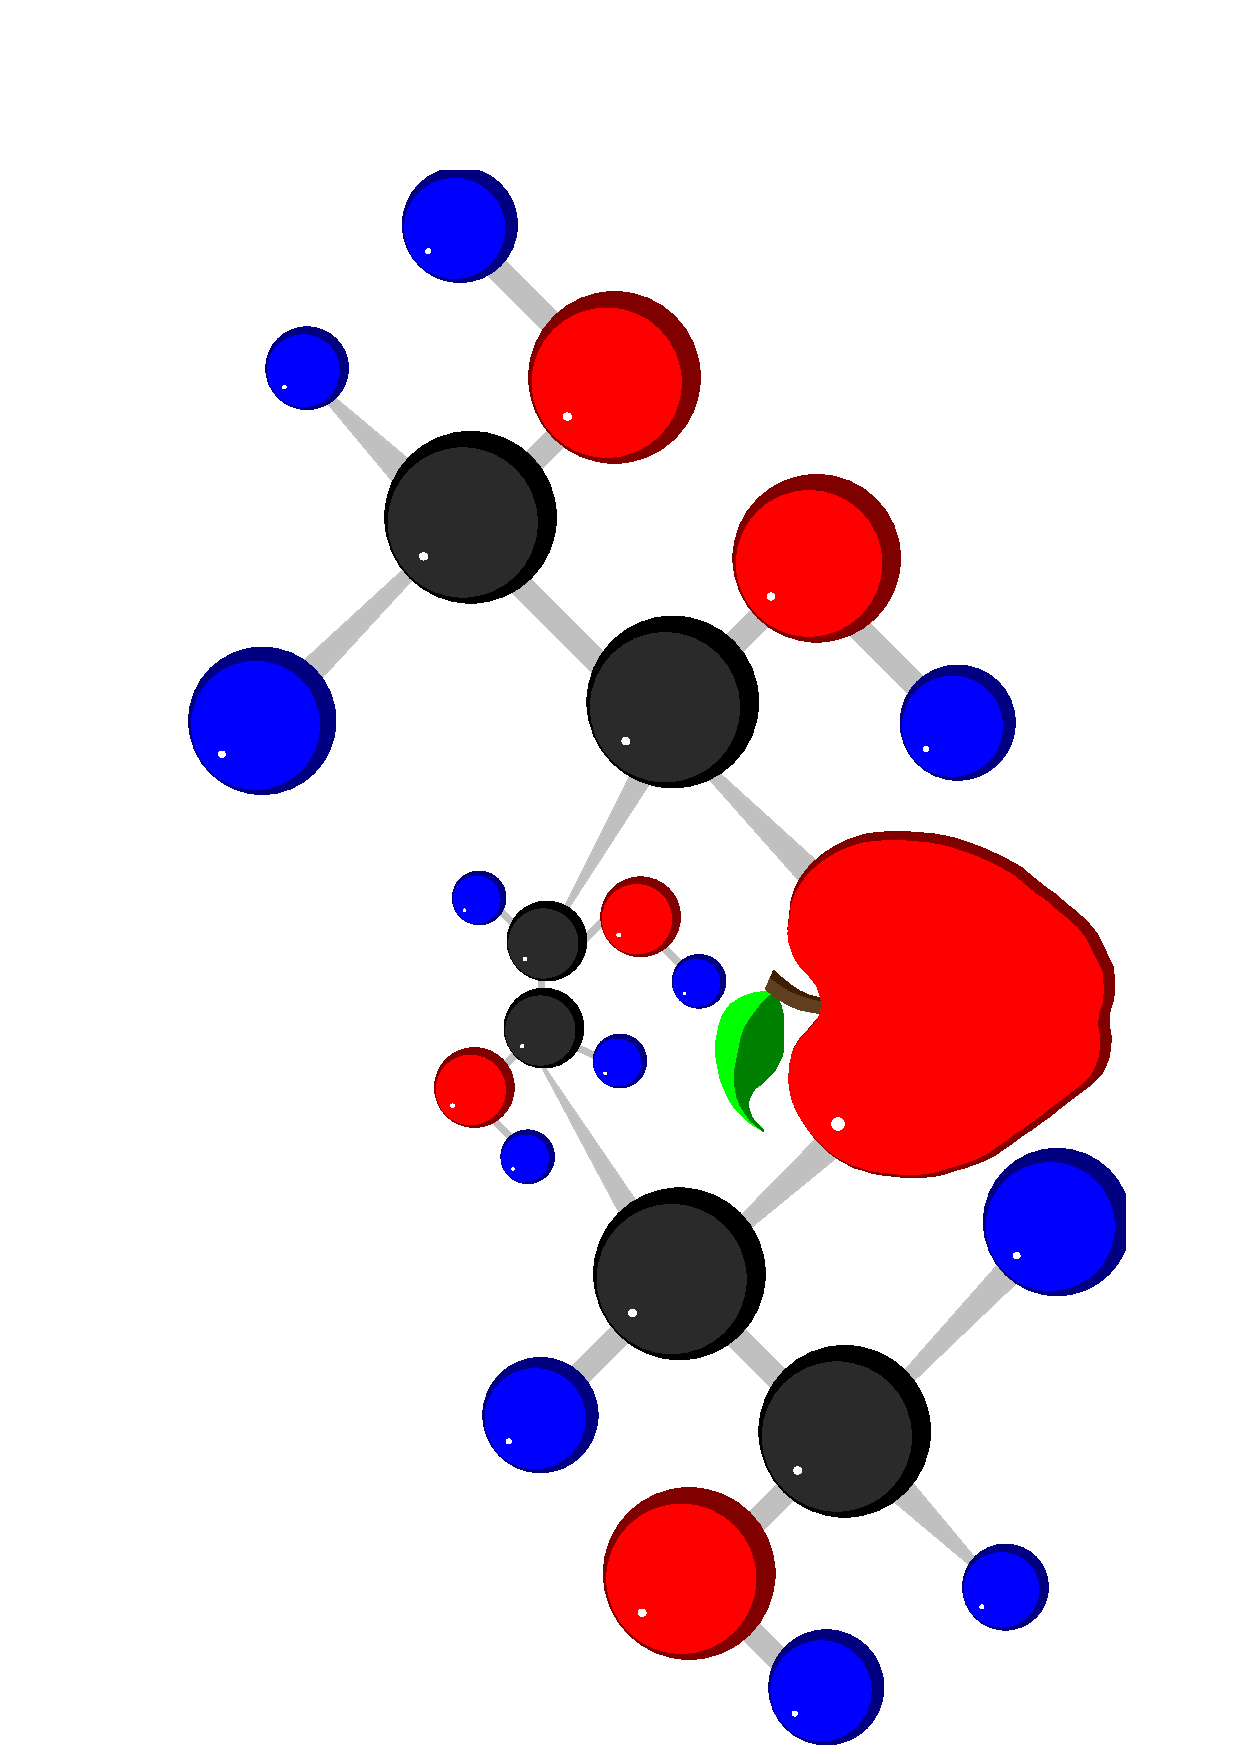
\includegraphics[width=0.5\textwidth]{CoverLogo}}
\author{Andre Masella}
\date{\today{} -- \input{Revision.tex}\\ \includegraphics{Revision.png}}
\maketitle

\tableofcontents

\chapter{Introduction}

\section{Welcome}
This book started because most of our family recipes were not written down. Those that were, often had misleading or blatantly incorrect instructions. Those that were correct, were still cryptic asking for ``enough flour to make dough the right consistency''. A particularly good example is \seerecipe{Cookies:BreakfastCookies} which required ``2~heaping teaspoons'' of baking powder. First, these were not standard teaspoons, but kitchen serving teaspoons. The heap is supposed to be so large that it almost cannot be removed from the container. After some precise measurements with a scale, I found that these ``teaspoons'' were 3~times larger than a standard teaspoon.

I hope to slowly standardise the recipes and make the quantities sound. It is best to assume all quantities, if even present, are subject to judgement and revision. If you make a discovery about a quantity, please tell me and I will change this book.

Some recipes are marked \UNTESTED{} meaning I have not made them, but they seem sound even though they came from the Internet. Some recipes are marked with \FIXME{}. These are undoubtedly family recipes lacking quantities, having incorrect quantities, or having missing information. If you make one of these, please accurately measure the ingredients and help me update this book.


\section{Preparation}
This has been typeset using \href{http://www.ctan.org}{\LaTeX}, using custom recipe environments. The cover graphic was made in \href{http://www.inkscape.org}{Inkscape}. Revision control is done through \href{http://subversion.tigris.org/}{Subversion}.\par

\section{Conversion Hints}
It is good to know that: \par

\begin{tabular}{c c c c c c c}
\tp{3} & = & \Tp{1} & = & \oz{\half} & = & \C{$\sfrac{1}{16}$} \\
\C{1} & = & \oz{8} & = & \qt{\quarter} & = & \mL{250}
\end{tabular}

In this book, no distinction is made between fluid ounces and avoirdupois ounces~(mass) in writing. I hope to eventually replace all ounces with either grams or mL.

\section{Cooking Charts}

\subsection{Sugar Cooking}
\begin{tabular}{|lcc|}
\hline
Stage			& Temperature \tC{(}) & Temperature \tF{(}) \\
\hline
Pearl			& 104 to \tC{106} & 220 to \tF{222} \\
Thread			& 106 to \tC{112} & 223 to \tF{235} \\
Blow or Soufflé	& 110 to \tC{112} & 230 to \tF{235} \\
Soft Ball 		& 112 to \tC{166} & 234 to \tF{240} \\
Firm Ball 		& 116 to \tC{120} & 242 to \tF{248} \\
Hard Ball 		& 121 to \tC{129} & 250 to \tF{265} \\
Soft crack 		& 132 to \tC{143} & 270 to \tF{290} \\
Hard crack 		& 149 to \tC{154} & 300 to \tF{310} \\
Light caramel 		& 160 to \tC{170} & 320 to \tF{338} \\
Medium caramel 		& 176 to \tC{182} & 350 to \tF{360} \\
Dark caramel 		& 188 to \tC{204} & 370 to \tF{400} \\
Black Jack or Monkey's Blood	& \tC{210} & \tF{410} \\
\hline
\end{tabular}
\vspace*\fill

\subsection{Meat Cooking}
\begin{tabular}{|lllc|}
\hline
Meat		& Cut				& Taste		& Temperature \\
\hline
Beef and Lamb	& Roasts, Steaks and Chops	& Rare		& 120 to \tF{125} \\
		&				& Medium Rare	& 130 to \tF{135} \\
		&				& Medium 	& 140 to \tF{145} \\
		&				& Medium Well	& 150 to \tF{155} \\
		& 				& Well Done	&        \tF{160} \\
		& Ground Meat			&		& 160 to \tF{165} \\
Chicken and Duck	& 			&		& \tF{165} \\
Turkey		&				&		& \tF{165} \\
Pork		& Roasts, Steaks and Chops	& Medium	& 140 to \tF{145} \\
		&				& Well Done	& \tF{160} \\
		& Sausage (raw)			&		& \tF{160} \\
		& Ham (raw)			& 		& \tF{160} \\
		& Ham (precooked)		&		& \tF{140} \\
Fish		& Steaks, Fillets or Whole	&		& \tF{140} \\
Tuna, Swordfish, and Marlin &			&		& \tF{125} \\
\hline
\end{tabular}

A turkey's temperature can rise \tF{30} when resting.

\vspace*\fill

\subsection{Barbecue Cooking}
\begin{tabular}{|lllc|}
\hline
Meat					& Heat			& Taste		& Time \\
\hline
Hamburger~(\inch{\threequarter})	& Medium		& Medium	& 8 to 10~minutes \\
					&			& Well Done	& 10 to 15~minutes \\
Frozen Patties			 	& Low to Medium 	& Medium	& 12 to 14~minutes \\
Beef Steak~(\inch{1})			& Medium 		& Rare		& 3 to 6~minutes \\
					&			& Medium	& 6 to 9~minutes \\
					&			& Well Done	& 9 to 12~minutes \\
Beef Roast				& Low 			& Rare		& 12 to 15~minutes per lb \\
					&			& Medium	& 15 to 20~minutes per lb \\
					&			& Well Done	& 20 to 25~minutes per lb \\
Pork Chops~(\inch{\half})		& Medium		& Medium	& 8 to 10~minutes\\
					&			& Well Done	& 15 to 20~minutes\\
Pork Ribs~(3 to \lbs{4})		& Low to Medium		&		& 45 to 90~minutes\\
Pork Roast~(3 to \lbs{5})		& Low to Medium		& Well Done	& 18 to 23~minutes per lb\\
Lamb Chops~(\inch{\half})		& Medium 		&		& 6 to 12~minutes\\
Chicken~(2\half{} to \lbs{3\half})	& Low			&		& 75 to 90~minutes\\
Turkey/Chicken~(2 to \lbs{5})	 	& Medium/Low 		&		& 30~minutes per lb \\
Chicken--Halved or Quartered 		& Low 			& 		& 25 to 30~minutes\\
Chicken Breast (\oz{6}) 		& Medium	 	&		& 8 to 12~minutes\\
Boneless Chicken Breasts (Halves) 	& Medium 		&		& 10 to 12~minutes\\
Fillets~(6 to \oz{8}) 			& Medium to Hot 	&		& 8 to 12~minutes\\
Fish Steaks~(\inch{1})		 	& Medium to Hot 	& Well Done	& 10 to 15~minutes\\
Shrimp					& Low to Medium 	&		& 8 to 12~minutes\\
Baking Potato				& Medium 		&		& 25 to 30~minutes\\
Corn					& Low to Medium 	&		& 15 to 20~minutes\\
Zucchini--Halved 			& Medium 		&		& 6 to 10~minutes\\
\hline
\end{tabular}

If fish is frozen, brush with oil and double grilling time.

\vspace*\fill

\subsection{Cream Types}

\begin{tabular}{|l|rr|}
\hline
Cream Name		& Minimum Fat~(\%) & Maximum Fat~(\%) \\
\hline
Half \& Half 	& 10.5	& 18 \\
Table Cream		& 18	& 30 \\
Medium Cream 	& 25 	& \\
Whipping Cream	& 30	& 36 \\
Heavy Whipping Cream	& 36 & $+$ \\
Extra-Heavy Cream		& 38 & $+$ \\
\hline
\end{tabular}
\vspace*\fill

\subsection{Aromatic Combinations}
\begin{tabular}{|llp{4in}|}
\hline
Name & Origin & Ingredient Ratio\\
\hline
Mirepoix & French & \C{2} onion : \C{1} carrot : \C{1} celery \\
Mirepoix blanc & French & \C{1} onion : \C{1} parsnip : \C{1} celery \\
Battuto & Italian & bacon : garlic : onion : parsley : carrot : celery : green peppers~(optional) \\
Sofrito & Spanish & head of garlic : \C{2} bell peppers : \C{1} tomatoes : bunch of cilantro : small bunch of parsley \\
Trinity & Cajun & \C{2} onion : \C{1} green pepper : \C{1} celery \\
-- & Chinese & scallion : garlic : ginger : chili peppers \\
\hline
\end{tabular}

Aromatics generally form the basis of a dish, especially a soup or stew. They are usually sautéed with butter, oil, the fat render from the meat in the dish, or a combination. There is some flexibility and one aromatic combination may be substituted for another to change the flavour of a dish without leaving a ``hole''.
\vspace*\fill

\subsection{Fat Types}
\begin{tabular}{|llll|}
\hline
Name & Consistency & Origin & Processing\\
\hline
Fat & -- & Any & Any\\
Wax & Solid and Brittle & Plant & None \\
Shortening & Solid & Plant & Hydrogenated \\
Oil & Liquid & Plant & None \\
Lard & Solid & Animal & None \\
Grease & Liquid & Animal & None \\
\hline
\end{tabular}
\bigskip


The smoke point is the point where an oil smokes and beings to burn.


\noindent\begin{tabular}{|llc|}
\hline
Fat & Quality & Smoke Point \\
\hline
Almond oil & & \tF{420} -- \tC{216}\\
Avocado oil & & \tF{520} -- \tC{271}\\
Butter & & \tF{350} -- \tC{177}\\
Canola oil & Expeller Press & \tF{464} -- \tC{240}\\
Canola oil & High Oleic & \tF{475} -- \tC{246}\\
Canola oil & Refined & \tF{468} -- \tC{242}\\
Coconut oil & Unrefined & \tF{350} -- \tC{177}\\
Corn oil & Unrefined & \tF{320} -- \tC{160}\\
Corn oil & Refined & \tF{450} -- \tC{232}\\
Cottonseed oil & & \tF{420} -- \tC{216}\\
Flax seed oil & Unrefined & \tF{225} -- \tC{107}\\
Ghee (Indian Clarified Butter) & & \tF{485} -- \tC{252}\\
Grapeseed oil & & \tF{420} -- \tC{216}\\
Hazelnut oil & & \tF{430} -- \tC{221}\\
Hemp oil & & \tF{330} -- \tC{165}\\
Lard & & \tF{370} -- \tC{182}\\
Macadamia oil & & \tF{413} -- \tC{210}\\
Olive oil & Extra virgin & \tF{375} -- \tC{191}\\
Olive oil & Virgin & \tF{420} -- \tC{216}\\
Olive oil & Pomace & \tF{460} -- \tC{238}\\
Olive oil & Extra light & \tF{468} -- \tC{242}\\
Olive oil, high quality (low acidity) & Extra virgin & \tF{405} -- \tC{207}\\
Peanut oil & Unrefined & \tF{320} -- \tC{160}\\
Peanut oil & Refined & \tF{450} -- \tC{232}\\
Rice bran oil & & \tF{490} -- \tC{254}\\
Safflower oil & Unrefined & \tF{225} -- \tC{107}\\
Safflower oil & Semi-refined & \tF{320} -- \tC{160}\\
Safflower oil & Refined & \tF{510} -- \tC{266}\\
Sesame oil & Unrefined & \tF{350} -- \tC{177}\\
Sesame oil & Semi-refined & \tF{450} -- \tC{232}\\
Soybean oil & Unrefined & \tF{320} -- \tC{160}\\
Soybean oil & Semi-refined & \tF{350} -- \tC{177}\\
Soybean oil & Refined & \tF{450} -- \tC{232}\\
Sunflower oil & Unrefined & \tF{225} -- \tC{170}\\
Sunflower oil & Semi-refined & \tF{450} -- \tC{232}\\
Sunflower oil, high oleic & Unrefined & \tF{320} -- \tC{160}\\
Sunflower oil & Refined & \tF{450} -- \tC{232}\\
Tea seed oil & & \tF{485} -- \tC{252}\\
Vegetable shortening &  \tF{360} -- \tC{182}\\
Walnut oil & Unrefined & \tF{320} -- \tC{160}\\
Walnut oil & Semi-refined & \tF{400} -- \tC{204}\\
\hline
\end{tabular}
\vspace*\fill

\subsection{Flour Types}

The see of a plant contains three parts: the germ, the plant embryo; the bran, the hard outer shell; and the endosperm, the starch storage for the plant. All flours can be categorized by which of these they contain, how finely they are milled, and the source plant. Some flours go through bleaching to change the colour. There are different kinds of wheat: hard and soft. Hard, or winter, wheat contains a lot of protein, while soft, or spring wheat, contains less protein. Durum wheat is a specific strain of hard wheat. The different combinations are better at different tasks.


\noindent\begin{tabular}{|llllll|}
\hline
Name & Source & Components & Milling & Processing & Uses \\
\hline
All-Purpose & Medium Wheat & Endosperm & Fine & Bleached & Most Baking \\
Atta & Hard Wheat & All & Medium & None & Chapatis and Pasta \\
Brown Rice & Rice & All & Fine & None & Noodles \\
Buckwheat & Buckwheat & Varies & Fine & None & Noodles \\
Cake and Pastry & Soft Wheat & Endosperm & Very Fine & Bleached & Cakes and Pastries \\
Corn Flour & Corn & Varies & Fine & None & Bread and Tortillas \\
Corn Meal & Corn & All & Coarse & None & Muffins and Cornbread \\
Cracked Rye & Rye & All & Very Coarse & None & Bread \\
Dark Rye & Rye & All & Medium & None & Bread \\
Durum & Hard Wheat & Endosperm & Medium & None & Bread and Pasta \\
Graham & Medium Wheat & All & Mixed & None & Crackers \\
Gram & Chickpeas & All & Medium & None & Breading \\
Light Rye & Rye & Endosperm & Medium & None & Bread \\
Masa de harina & Corn & Varies & Fine & Nixtamalized & Bread and Tortillas \\
Rice & Rice & Endosperm & Fine & None & Noodles \\
Semolina & Hard Wheat & Endosperm & Coarse & None & Pasta and Bread \\
``Smart'' & Medium Wheat & All & Fine & Bleached & All-Purpose Replacement \\
Unbleached & Hard Wheat & Endosperm & Fine & None & Bread \\
Whole Wheat & Medium Wheat & All & Fine & None & Miscellaneous Baking \\
\hline
\end{tabular}

Durum flour is available at the Bulk Barn. Corn flour refers to corn starch in Britain; when corn flour is mentioned here, use the Spanish or Portuguese brands.

\subsection{Potato Types}
\begin{tabular}{|ll|}
\hline
Name & Class\\
\hline
Russet & Mealy\\
Goldrush & Mealy\\
Long White & Mealy\\
Idaho & Mealy\\
Yukon Gold & In-between\\
Peruvian Blue & In-between\\
Superior & In-between\\
Kennebec & In-between\\
Kathdin & In-between\\
Red-skinned & Waxy \\
White & Waxy \\
Crescent & Waxy \\
Yellow & Waxy \\
\hline
\end{tabular}

A cured potato has a thick skin while a new potato has a thin one. Normally, ``new potatoes'' are new white potatoes.

Potatoes~(\textit{Solanum tuberosum}) and sweet potatoes~(\textit{Ipomoea batatas}) are only distantly related. Although sweet potatoes are called ``yams'', that refers to a more distantly related plant, \textit{Dioscorea}~sp. Sweet potatoes are actually most closely related to common morning glories~(\textit{Ipomoea purpurea}). They are usually acceptable substitutes for potato, except for the skin, as the ``in-between'' type.

\noindent\begin{tabular}{|ll|}
\hline
Class & Uses\\
\hline
Mealy & Baking\\
      & Mashing\\
      & French fries\\
      & Baking\\
In-between & Gnocchi \\
           & Perogies \\
Waxy  & Soups and Stews \\
      & Salad \\
      & Casseroles \\
      & Roasting \\
      & Barbecuing \\
\hline
\end{tabular}

In-between varieties can do the jobs of mealy or waxy potatoes, but not as well. Mealy potatoes become light and fluffy when cooked, but tend to fall apart. Waxy potatoes keep their shape, but become lumpy when mashed. Yukon Gold is particularly good for gnocchi and perogies because it can be mashed smoothly (like a mealy potato), but does not absorb much water (like a waxy potato).

\vspace*\fill

\subsection{Pastry Methods}
Most doughs fall into one of the following methods. Although some recipes vary, most will be roughly the same and making changes will produce predictable results (e.g., creaming more in the cake method will produce fluffier cake). If you have a ``recipe'' which is only a list of ingredients, just apply the appropriate method.

When fats are involved, different recipes will require fat as a liquid, soft solid, or hard solid. If the fat is an oil or melted, treat it as a liquid. If it is ``softened'' or room-temperature, it is usually worked in to dry flour and allowed to coat the flour to create a tender dough. If it is cold, it will create layers in between bits of flour to create a flaky texture. In this final case, having a metal pan in the freezer can be a way to quickly chill dough if it heats up during working. Some doughs, like pie crust, will have some soft solid and some hard solid to be both tender and flaky.

\subsubsection{The Muffin Method}\label{method:Muffin}
The muffin method is often used to prepare muffins and quick-breads.

\begin{enumerate}
\item Combine the dry ingredients. Usually, sifting is suggested. Sifting can be replaced by a trip through a food processor or vigorous whisking.
\item Combine the liquid ingredients and the eggs.
\item Melt the fat and add to the liquid ingredients.
\item Combine the wet and dry ingredients with a minimum of stirring. It \textbf{will} be lumpy and there \textbf{will} be some bits of dry ingredients.
\end{enumerate}

Excessive stirring will cause the over-development of gluten. This would result in a smaller, less tender muffin with tunnels and a peaked crust. 

\subsubsection{The Biscuit Method}\label{method:Biscuit}
The biscuit method is used to prepare biscuits and dumplings.

\begin{enumerate}
\item Combine the dry ingredients.
\item Combine the liquid ingredients and the eggs.
\item Cut the fat into the flour mixture until the mixture has a coarse texture.
\item Combine the wet and dry ingredients. Be careful not to over-mix. Once a ball of dough forms, it can be kneaded briefly.
\end{enumerate}

Cutting the fat into the flour will cause layers to form through the dough. These layers are what makes a biscuit flaky. Again, be aware that over-working the dough will result in biscuits that are less tender and flaky than they should be.
 
\subsubsection{The Cake or Creaming Method}\label{method:Creaming}
The cake method is used mainly for cookies and cakes.

\begin{enumerate}
\item Cream the fat and sugar together.
\item Beat the eggs then add to fat and sugar mixture and beat well.
\item Add the sifted dry ingredients alternately with the liquid ingredients, beginning and ending with the dry ingredients. After each addition, stir to combine the ingredients then beat briefly.
\item Fold in any flavourings, fruits, and nuts.
\end{enumerate}

Creaming the fat with the sugar and then with the eggs incorporates a lot of air, making the final product fluffy. While over-beating is still a possibility, the fat will help to prevent tough gluten from forming.

\subsubsection{The Bread Method}\label{method:Bread}
The bread method is used for most yeast risen breads, pizza dough, pretzels, and cinnamon buns.

\begin{enumerate}
\item Bloom yeast, if using active-dry yeast, using some warm water and sugar. The sugar should only be about \Tp{1} per \C{1} water.
\item Combine the dry ingredients. If using volumetric measurements, reserve some of the flour.
\item Combine the liquid ingredients.
\item Add yeast to liquid ingredients.
\item Stir until stiff.
\item Knead until dough passes the window pane test. The test is performed by gently stretching the dough. If the dough can be stretched thin enough for light to pass through without tearing, the dough is done. If the dough is too sticky, the reserved flour can be added sparingly; a dough which is too moist is usually better than a dough which is too dry. Over-kneading is possible, but nearly impossible by hand and unlikely using a mixer.
\item Let ``ferment'' (first rise), usually, until doubled in bulk. This takes, in most recipes, 1 to 2~hours. Sometimes, this step is done in a refrigerator, in which case it is ``retarded'' and this takes over night.
\item ``Turn'' (deflate or punch-down) the dough by folding the dough like a letter and flattening with finger tips. The purpose is \textbf{not} to remove every gas bubble from the bread.
\item Let ``proof'' (second rise). This rise may also be ``retarded''.
\item Infrequently, the dough maybe turned and proofed again. Each subsequent cycle will take longer than the previous one.
\end{enumerate}


\vspace*\fill

\subsection{Yeast Types}
For bread baking, most commonly used yeast is \textit{Saccharomyces cerevisi\ae}, commonly called baker's yeast or brewer's yeast. It is capable of digesting many sugars as a food source including the maltose produced by the break down of starch in the flour. The types of yeast below are listed from most potent to least potent. The can all be substituted for one another if the quantity is adjusted. If too much yeast is added, the final product will taste of yeast and too little will rise prohibitively slowly. Yeast grow optimally at \tC{30} and will die if exposed to temperatures greater than \tC{40}.

\begin{description}
\item[Compressed Yeast] -- Yeast is sold in a beige block which is firm to the touch but crumbles when pressed. Also referred to as live yeast, fresh yeast, or a yeast cake. It has a short shelf life of only a month in the fridge and risks growing mould. It can be frozen, ideally in a deep freezer and should not be defrosted repeatedly. It can be crumbled directly into dough or dissolved in water. A ``cube'' is \gr{25}.
\item[Instant Yeast] -- Yeast is sold in granules that have a very long shelf life. The most common brand is Fleischmann's. Also referred to as Rapid-Rise or Quick-Rise. It does not need to be ``activated'' before use, but it should be dissolved in water. Activating it does no harm. It can be stored unopened for 1~year; once opened, 3~months if stored in the fridge or 6~months in the freezer.
\item[Active Dry Yeast] -- Yeast is sold in granules that have a fairly long shelf life. Instant yeast has effectively replaced active dry. One can be substituted for the other, but less instant is required. Yeast must be ``activated'' by mixing with warm sugar water and allowing to stand for 10~minutes. It can be stored unopened for 1~year; once opened, 3~months if stored in the fridge or 6~months in the freezer.
\item[Sourdough Starter] -- Naturally occurring yeast, usually \textit{Saccharomyces cerevisi\ae}, \textit{Saccharomyces exiguus}, and/or \textit{Candida} sp.,  and lactic acid bacteria are present in a piece of dough. Also referred to as a sponge. The starter is ``fed'' and some is used for baking and some is reserved for future use. Starter can be kept in the fridge for months if no mould grows, but is ideally fed at least every other week. If substituting, some of the water and flour in the recipe must be substituted for starter. If more than half of the water comes from the starter, the final bread will be sour.
\end{description}

Conversion can be done as follows:

\begin{itemize}
\item Instant $\to$ Compressed : $\times 3$
\item Active Dry $\to$ Compressed : $\times 2.5$
\item Instant $\to$ Active Dry : $\times 1.25$
\end{itemize}

Osmotolerant yeast is a type of yeast bred to survive the high osmolarity (i.e., high sugar and salt concentrations) of sweet breads. Other forms of yeast will not raise the bread sufficiently without imparting a yeast flavour due to a need for more yeast to be added. It can be purchased in the US in an instant form.

\section{General Tips}
\begin{itemize}
\item Water in a stainless steel pot should be salted after boiling as the salt will corrode and pit the metal.
\item Before making a substitution, consult The Cook's Thesaurus~(\url{http://www.foodsubs.com/}).
\item There are two kinds of ice-cream: New York-style and Philadelphia-style. New York-style has a custard (i.e., egg base) and is cooked. Philadelphia-style has no eggs and is usually uncooked. The difference gives New York-style a very rich and heavy flavour while Philadelphia-style is usually more light and fruity.
\end{itemize}

\noindent Pasta Specific Tips:
\begin{itemize}
\item Dishes from the ``Pasta'' category must be served immediately, while dishes in the ``Pasta Sauce'' can be made ahead of time and frozen.
\item When removing meat from pasta sauce, a small well of pasta water should be added to ``rinse'' the meat as it is being removed.
\item When dressing pasta Nonna-style, toss the pasta with half the cheese and half the tomato sauce, put into individual dishes, sprinkle remaining cheese and ladle remaining sauce on top. Adding sauce with cheese on top is ``ristorante''-style.
\item If substituting canned tomatoes, diced tomatoes are equivalent to tomato pieces in most recipes and crushed tomatoes are equivalent to purée.
\item Rice may be substituted for pasta in many dishes by boiling the Arborio rice in a large volume of salted water.
\end{itemize}

\noindent Bread Specific Tips:
\begin{itemize}
\item To raise bread faster, put the bread in a cold oven with a bowl or pot of boiled water. Reheat the water when it cools.
\item To make a firmer crust on breads, increase the oven temperature and steam the oven by cracking the door and wetting the sides of the oven with a spray bottle of water or dropping ice cubes in a pan with rocks.
\item The oven should be preheated \tF{50} above the target temperature to compensate for the heat lost when the oven door is opened to insert the bread.
\item Starter, whisked down, has a density of \gr{300} per \C{1}.
\item According to Alton Brown, bread should be cooked until it reaches an internal temperature of \tF{207}. Any higher than \tF{210} and the water inside the bread will boil causing the bread to boil. Lower than \tF{205} will result in under cooked yeasty-flavoured bread. Times are suggestions based on experience before cooking by temperature or for recipes where inserting a temperature probe is not practical. Any recipes where bread is not cooked to \tF{207} are explicitly labelled. If a bread has reached \tF{207} but the crust is not dark enough, decrease oven temperature by \tF{50} and watch that the internal temperature does not exceed \tF{210}. The temperature probe should not be inserted until the crust forms. Allow the bread to bake for 10~minutes before inserting the meat thermometer.
\item Starter should be grown in glass, plastic, or stainless steel vessels.
\item Malt extract syrup and malt extract powder can be interchanged. Malt syrup is 20\% water and the powder has no water. Adjust the water in the recipe appropriately.
\end{itemize}

\noindent Emergency Tips:
\begin{itemize}
\item If the oven is not working, place a cake in a large pot raised off the bottom using a metal rack, trivet, or jar lids. Add water to the pot and steam the cake. Cook for the usual length of time.
\item If you do not have an ice cream maker, you can freeze the ice-cream solid, cut it into cubes, and use a blender to liquefy the cubes, then freeze the mixture. This method will never produce ice crystals as small as a real ice-cream maker, but the final product will be fairly smooth.
\end{itemize}

\importrcp{rcp:ToastingNuts}{ToastingNuts}
\importrcp{rcp:PseudoFrying}{PseudoFrying}

\mainmatter

\chapter{Dip}


\backmatter

\chapter{Glossary}
\begin{description}
\item[baccalà] \pronounce{bahk-kah-LAH} --- Dried salted cod.
\item[banneton] --- A round wicker basked lined with a linen cloth. Substitute a self-standing colander with a cotton teatowel. The Italian way is to wrap the bread in a loose packet and then flip it so the ends are underneath; as the bread rises, it will inflate the packet making it firm.
\item[ciúlisë] \pronounce{chu-LISH} --- The cooking water from pasta.
\item[grigne] \pronounce{GREEN-yuh} --- The slash marks in the top of a loaf of bread.
\item[pëpparulë] \pronounce{peh-pa-ROOL} --- Sweet red pepper flakes. Substitute paprika.
\item[squiccëlë] \pronounce{skwi-CHEH-leh} --- The arbitrary amount of oil needed by recipes that do not specify a quantity of oil. Approximately 1 to \Tp{3}.
\item[window-pane test] --- A test to see if bread is sufficiently kneaded. Stretch a small section of bread gently. If the bread can be stretched thin enough for light to pass through with out tearing, the dough is ready.
\end{description}

\printindex

\appendix
\chapter{Stealing Recipes}
My grandparents cook without recipes. Getting them to give you a recipe is almost impossible; even getting a list of ingredients can prove challenging. I have gained experience in how to extract recipes from them. I will share my secrets and describe my method.

\section{Invitation}
The only way to get the recipe is to watch them do it and observe what they do and write it all down.

The first decision to make is location. There are pros and cons to doing it in their kitchen versus yours. In their kitchen they have the tools they are used to. They may have a favourite cup to measure flour or be able to estimate in their pans. Taking them out of their element will be disruptive to their cooking. However, they will often focus more in your kitchen. I know my grandparents are constantly working on many things at once. It becomes unclear if something is sitting on the counter because it needs to sit or because something else needs attention.

If you are going to do it in their home, you're going to need to bring some of your own tools. I recommend the following:

\begin{description}
\item[Notebook and pen] --- This is where you will write down your observations. I find that writing on papers gets lost, so I have a section of a notebook dedicated to this. A smaller notebook is better since it will be more unobtrusive when working. Make sure it is reasonably rugged since it will get covered in food.
\item[Calibrated Measuring Devices] --- If my grandmother says she has teaspoons, she means the things you stir your tea with, not the calibrated measuring spoons. Bring some of those and some cups.
\item[Scale and calculator] --- Measuring by weight is the best way to reduce variability in the recipe. Since there will probably be arithmetic involved to make use of the scale's amounts, I suggest a calculator.
\item[Funky Hardware] --- If the dish requires some funky hardware, like the board for gnocchi, the fi\'err\"e for maccarun\"e, bring it to have it approved. If you don't have one of these thingies, you should start looking. They will probably tell you they got theirs from Old Country before the war, so you'll have to find an equivalent. You'd be amazed what is available at resturuant supply stores. Also, ethic stores, Chinatown, dollar stores, and hardware store all might carry the thing you need or something functionally equivalent. Be warned, they'll never know it by the same name, so you must browse. You can also try the Google. Another person may have posted this question to a forum. Sometimes, you have to really think: I could not find a fiérrë, a small square rod, to make maccarunë, so I went to talk to a machinst and he told me to look for key stock. That was easy to find.
\item[Watch] --- For timing, since they don't.
\item[Instant-Read Thermometer] --- This is not always necessary, but for frying, it's nice to know the oil temperature. It can also be useful for certain meats, but since my grandparents like to overcook meat, I don't bother. It is probably useful in stove-top braising, poaching, and other sub-boiling techniques.
\end{description}

\section{Everything is Important}
Assume everything they do is important. Most of it isn't. In fact, much of it is probably pointless. For now, get it all down. If you can make this dish multiple times and take an average, so much the better. This is an important distinction: \emph{don't write anything they tell you}. Write what you observe. They may tell you things that are misleading or just plain wrong. It's probably not intentional. If you want to write it down, note that it was not observed.

Be as precise as possible. If you know the cooking vocabulary, use it. Putting oil and garlic in a pan can be a sauté or a sweat depending on the temperature. If you don't know the difference, write down what setting the stove is at. Does the garlic blister? colour? Is it covered in oil? Is it in a shallow pan? non-stick pan? Is the garlic minced? crushed? halved? Imagine describing it to someone who is not in the room.

Take every opportunity to do instead of watch. If dough is involved, touch it, squeeze it, and stretch it. If dough is not something you handle frequently, bring some modeling clay or cheese wax and try to describe the dough relative to those.

Examine ingredients thoroughly. Write down brand names and, if you aren't familiar with them, find out where they get them. My grandmother has very specific rules about which brands of flour she uses for what. She doesn't understand why, but some are better. What she is really looking for is the amount of protein in the flour. Robin Hood All-Purpose flour has lower protein content than Five Roses All-Purpose, making the Robin Hood better suited to cake and pastry and the Five Roses to pasta. Ask if they always use this brand.

\section{How to Measure}
	Measuring ingredients is hard. If you have a scale, I would measure everything by weight. Even if you want a recipe by volume, a scale is convenient because you can shove it under their work bowl and just keep measuring. If you are measuring by volume, you'll just have keep shoving cups under their hands and measuring before they drop it into the bowl. My grandmother's pasta was particularly annoying because she would make it too wet, then add flour, then it would be too dry and she would add more water. My solution for that particular recipe was the weigh the bag of flour before and after and weigh the dough at the end. Then I could calculate the amount of flour and water in the dough.

Measuring time is fairly easy. Just remember to do it.

\section{Quantifying the Measurements}
The question I ask most frequenty is ``what are you looking for?''. That is the golden question. This is most important during the cooking. Given they don't time, what are they looking for? Is it the colour? smell? cracks? puffing? This is also important in doughs and batters. How do you know it is kneaded enough? stickiness? smoothness? colour?

If you are learning a technique, after you've rolled or folded a few whatevers, describe what you are doing to them in different words and see that they are satisfied. This can be especially important if there is a language barrier.

Don't ask why. The probably don't know or their answer is wrong.

\section{Fixing the Recipe}
Once you have observed it, come home and immediately rewrite it in a ``standard'' recipe format. Do any calculations you need for you ingredients. If you measured in weight but want volume, use your scale to convert by measuring the same weight in a calibrated container. If there is a strange technique, like rolling maccarunë, write it down in a detailed set of steps. Draw pictures if it helps. It is important to do this while it is fresh in your mind.

Try to make it. Make it with all the strange and seemingly pointless steps. If you get something pretty darn close, you may begin whittling; if not, make it again and, if that fails, observe again. There is also a lot of variablility in their cooking. If it consistently comes out to watery, assume your measurement is off and decrease it.

The recipe at this point is full of seemingly useless steps or things that are way too complicated. Pick something that seems illogical or laborious and change it. If your change works, keep it. Keep whittling down the recipe until you think it is manageable. In some recipes, I have taken the opposite approach. I have stripped the recipe down to what I think are essential steps and added steps back. Some steps require patience to get right. After years, we are still learning how to make a frittata. It can be very hard to tell non-sense from critical steps. Kneading the ground beef in meat balls changes the texture. Pressing down calzone makes them fluffier. I didn't know that until I took them out of the recipe. Besure to log your subsequent attemps in your notebook. If skipping a step makes it chewy, it's the only way you'll know.

In parallel, you can also start changing the ingredients. My grandmother's dishes tend to be extremely high in fat. A lot of times, this can be drastically reduced without changing the dish substantially. You can also see if the particular brands they use are better suited to this recipe than others.

\section{The Ultimate Test}
The final challenge for your newly transcribed recipe is to make it for them. If it gets the seal of approval, it's a keeper.

\section{Peasant Cooking}
Most of the recipes I've tried to capture are peasant dishes made when people had a fair amount of time on their hands. Really, one must have been pretty bored to consider rolling stuff in a cabbage leaf. There are two hallmarks of peasant cooking: intricate steps and long cooking times.

Intricate steps are probably unavoidable. Making cabbage rolls or maccarunë are going to be extremely laborious just because of the effort required to form each one. I try to remind myself that if it was winter in the Ukraine before TV, I'd probably be pretty bored too. That being said, there are cheats. Cabbage roll casserole made like a lasagna tastes pretty much the same and tagliatelle made with a pasta machine are much better than any store bought pasta.

Long slow cooking times are definitely unavoidable. Long slow cooking times are not a product of too much time. They are a necessary way to tenderise meats and extract flavours. Long gentle cooking causes connective tissue in meat to break down. Even though we may have better ingredents now, a long slow cook will always make for more tender meat. It's also important to remember that water is a solvent. Cooking soup for hours is necessary because that is the time needed to extract the flavours from the ingredients. If you want to make things quicker, don't resort to increasing the heat and shortening the cooking time. The answer is more likely in technology. Would it be better in a pressure cooker? slow cooker? Can you make a huge batch and freeze it fully cooked? prepared but uncooked? ingredients prepped? some ingredients? Another technique to note is a braise: a long slow cook just below a simmer. My grandparents always did it on the stove top, which requires constant fussing with the temperature. Instead, you'll probably want to braise in the oven, a slow cooker, or a pressure cooker. If you cook too hot, your dish will never tenderise the same way.

It's also important to understand that somethings have changed. My grandparent cook pork to shoeleather, but their reason was good. When they were growing up, most pigs were fed scraps and the meat was frequently contaminated with trichinosis. Grocery-store pork is fed grain and regulated so it doesn't contain trichinosis, therefore doesn't need to be cooked as much.

\section{Closing}
There's a joke I like: A recently married woman makes a ham for her husband. He says that it is fantastic, but asks why she cut the ends off. She replies that her mother made great ham and she always cut the ends off. They call her mother and ask why she cuts the ends of her ham. In turn, she says that her mother made great ham and she always cut the ends off. They then call her grandmother and inquire why she cut the ends of her hams. The grandmother says that she never had a pan big enough.

Good luck!

\chapter{Microbiology}
Sourdough and cheese recipes require some ``real'' microbiology work. These are derived from laboratory procedures and some laboratory equipment.
\begin{multicols}{2}\raggedcolumns
\section{Aseptic Technique}
Microbiology work requires ``aseptic technique'' which is a work method to prevent contamination so that only a single microorganism will be cultivated. Proper technique is not possible or necessary in the kitchen. In general, the following must be observed:
\section{Glassware}

For yeast, the ideal growing environment is a vented Erlenmeyer flask on a magnetic stirrer. The stirring helps aerate the media as yeast prefer to be oxygenated. If not available, it can be skipped, but the flash should be swirled occasionally. Special vented caps are available to allow air to flow into the flask but prevent dust from contaminating the culture. If not available, cover with a piece of aluminium foil. If an Erlenmeyer flask is not available, use any glass vessel with a narrow neck.

For cheese, the ideal growing environment is a sealed Erlenmeyer flask. If on a magnetic stirrer, soft cheeses like \seerecipe{Cheese:Quark} will be smoother. If this is not available, run the final product through a blender to remove any crystalline lumps. If a stoppered flask is not available, any clear sealed glass container will work. Beware of odour transfer between the cheese and the rubber seal of a jar.

\begin{itemize}
\item Clear all equipment thoroughly before using. Do not use soap unless needed and rinse extremely thoroughly.
\item Sterilise items by processing in a covered water bath for at least 30~minutes.
\item Items which are coming in direct contact with media can be quickly sterilised by dipping in alcohol and then being lit. Allow to cool momentarily before touching living cells.
\item Do not let equipment, especially the insides caps and stoppers, contact the counter.
\item Work quickly.
\item The major source of contamination is you. Do not allow a surface you have touched to contact a clean surface.
\end{itemize}

\importrcp{rcp:Osmotolerant}{Osmotolerant}
\importrcp{rcp:FrozenStock}{FrozenStock}
\end{multicols}
\end{document}
